%/*****************************************************************************
% * WindNinja Tutorial 1%/*****************************************************************************
\documentclass[12pt]{article}
%\documentstyle{report}
\usepackage{float}
\usepackage{graphicx}
\usepackage[margin=1in]{geometry}
%\usepackage{subfig}

\graphicspath{{imgs/}}

\usepackage[utf8]{inputenc}
\usepackage[english]{babel}
\usepackage[parfill]{parskip}
\usepackage{datetime}
\usepackage{hyperref}
\hypersetup{
	colorlinks=true,
	urlcolor=blue,
  }
\urlstyle{same}
%\newdate{date}{26}{04}{2018}
%\date{\displaydate{date}}
\usepackage{subcaption} 
\usepackage{dirtytalk}
\usepackage{multirow}
\usepackage{booktabs}


\usepackage{fancyhdr}
\pagestyle{fancy}
\fancyhf{}
\rhead{WindNinja Tutorial 1: The Basics}
\cfoot{\thepage}

\newcommand\vn{3.6.0}

\begin{document}
\begin{titlepage}
    \centering
    {\Huge
        WindNinja Tutorial 1:
        The Basics
    }    
    \vfill
    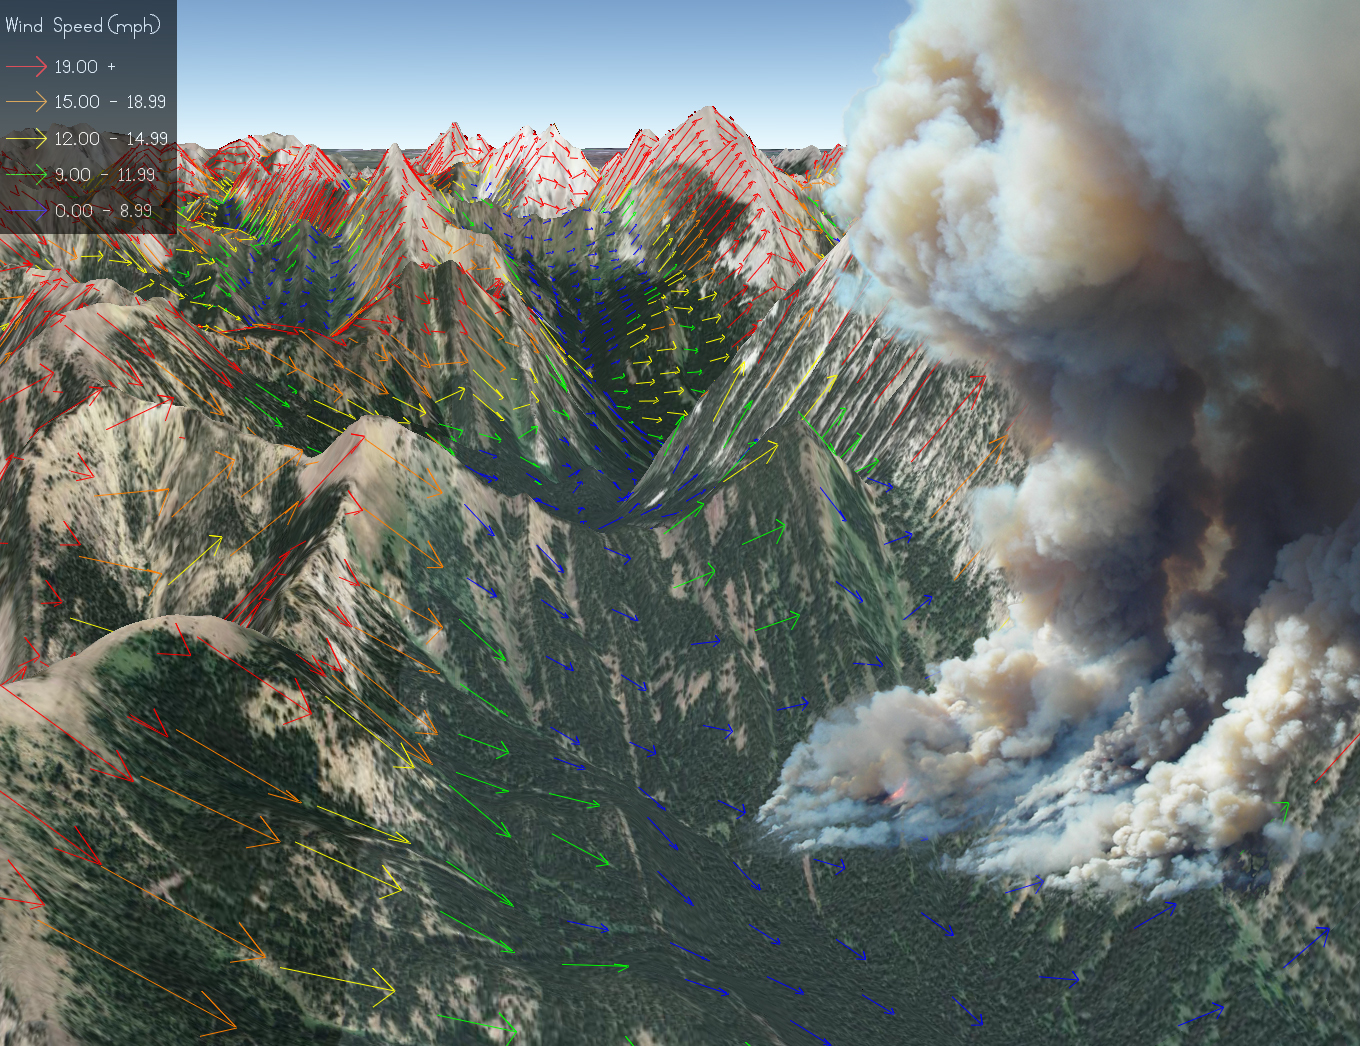
\includegraphics[scale=0.35]							{title_fig.jpg}
    \vfill
  	{\Huge
	  11/07/2024 %Date Last Edited
  	}
    \vfill
\end{titlepage}

\section*{Introduction}
\noindent
Welcome to \textbf{WindNinja Tutorial 1: The Basics}.  This tutorial will step you through the process of running a basic WindNinja simulation, including how to obtain the necessary elevation data for your specific area.  A basic WindNinja simulation uses a single input speed and direction to initialize and drive the wind flow.  More advanced topics such as diurnal wind simulation, atmospheric stability, weather station initialization, and weather forecast model initialization are discussed in other tutorials.  This tutorial covers both the “button pushing” part of running a simple simulation, as well as an understanding of the simulation process.  After the tutorial, you should feel comfortable obtaining elevation data, running WindNinja, and using and viewing the wind outputs.
\newline\break
Note:  All required user actions in this tutorial are shown in     \textbf{\color{red} red}.

\section*{What is WindNinja?}
WindNinja is a computer program that computes spatially varying wind fields for wildland fire applications.  It is specifically designed to simulate the effect of terrain on wind flow.  Unlike traditional weather models, WindNinja does not predict wind for future times, rather it simulates the spatial variation of wind for one instant in time (it does not step forward in time).  Information from standard textual weather forecasts can be used to help determine the inputs to WindNinja.  WindNinja has the ability to automatically obtain the necessary information from standard weather forecast models to do runs.  Using this method, WindNinja can essentially provide a forecast in time, since it does a WindNinja simulation for every forecast time step of the weather forecast model.  This is discussed in detail in Tutorial 4.  Also, because WindNinja is designed to account for the effect that terrain has on wind flow, it normally runs at a finer resolution (usually around 100-200 meter resolution) than traditional weather models (around 3 kilometer resolution or greater) so the terrain can be more fully resolved (individual ridges and valleys).

WindNinja has been designed so that a small number of user inputs are required, making simulations easy for non-specialists.  The inputs for a basic run are:  an elevation data file for the modeling area, a domain-averaged input wind speed and direction, and specification of the dominant vegetation in the area.  If you aren’t a GIS person, don’t worry!  WindNinja can be run by a person with zero GIS skills and no need to use a complicated GIS.  Also, simulations using WindNinja are fairly convenient since a simulation usually takes only a few seconds of run time.

Outputs from WindNinja can be used for viewing wind flow on maps and for incorporation into fire simulation models.  For viewing wind flow, several options are available to the user.  Probably the most convenient is to use the free version of Google Earth (using the wind output *.kmz file).  Other programs that can be used to view wind flow are GIS programs such as ArcView and ArcGIS (using the output *.shp shapefile), or FlamMap (using the output *.asc grid files).  WindNinja winds can be used in the fire spread programs FARSITE and FlamMap (using the output *.asc grid files and *.atm atmosphere files) and have been shown to increase fire spread simulation accuracy (see the publications \href{http://firelab.org/project/windninja}{here}).

Some users may recall a similar model called WindWizard. WindWizard provided a similar user experience but included more sophisticated physics. The physics in the WindWizard solver were based on proprietary software that required users to purchase a license. Because this severely hampered usability, WindWizard is no longer available. Instead, WindNinja has been upgraded to include the advanced physics previously included in WindWizard, but without the licensing fees.

As of version 3.0, WindNinja includes an optional momentum solver that replaces the functionality of WindWizard. There are now two options for the solver (the number-crunching part of WindNinja): 1) conservation of mass and 2) conservation of mass and momentum. The conservation of mass option is the native, fast-running solver used in previous versions of WindNinja. The conservation of mass and momentum option is a new solver based on the OpenFOAM toolkit. OpenFOAM is free, open-source software for computational fluid dynamics (CFD) from the OpenFOAM Foundation: \url{http://openfoam.org}. 

The major differences, from a user’s perspective, between the two solvers are listed below:

\begin{itemize}
\item The conservation of mass solver runs much faster than the conservation of mass and momentum solver (less than a minute for conservation of mass compared to about 10-30 min for conservation of mass and momentum).
\item The conservation of mass solver's approximation of the momentum equation is simpler and, at times, less accurate than that of the conservation of mass and momentum solver. This is mainly why the conservation of mass solver runs so much faster than the conservation of mass and momentum.  The conservation of mass simulations are normally less accurate during stronger winds on the lee sides of ridges and mountains where recirculation eddies can occur.
\item The conservation of mass solver incorporates some non-neutral atmospheric stability effects, while the conservation of mass and momentum is only valid under near-neutral stability.
\item WindNinja has a feature that allows users to enter measured wind information at several locations to drive the flow.  WindNinja will produce a wind field that matches the winds as these locations.  This feature is not currently available for the conservation of mass and momentum solver.\end{itemize}

\section{Getting Started}

You can download the WindNinja installation file from \url{www.firelab.org}.  Step through the simple installation process to install WindNinja.

\textbf{\color{red}Once installed, you can start WindNinja by going to Start $\Rightarrow$ Programs $\Rightarrow$ WindNinja \vn\ $\Rightarrow$ WindNinja \vn\ }

The main WindNinja window will open.  In addition to the usual toolbar features at the top (File, Options, Tools, Help), the window consists of a navigation tree area, an input panel area, and a console output area as shown in the figure below.

\begin{figure}[H]
	\centering
	\label{}
	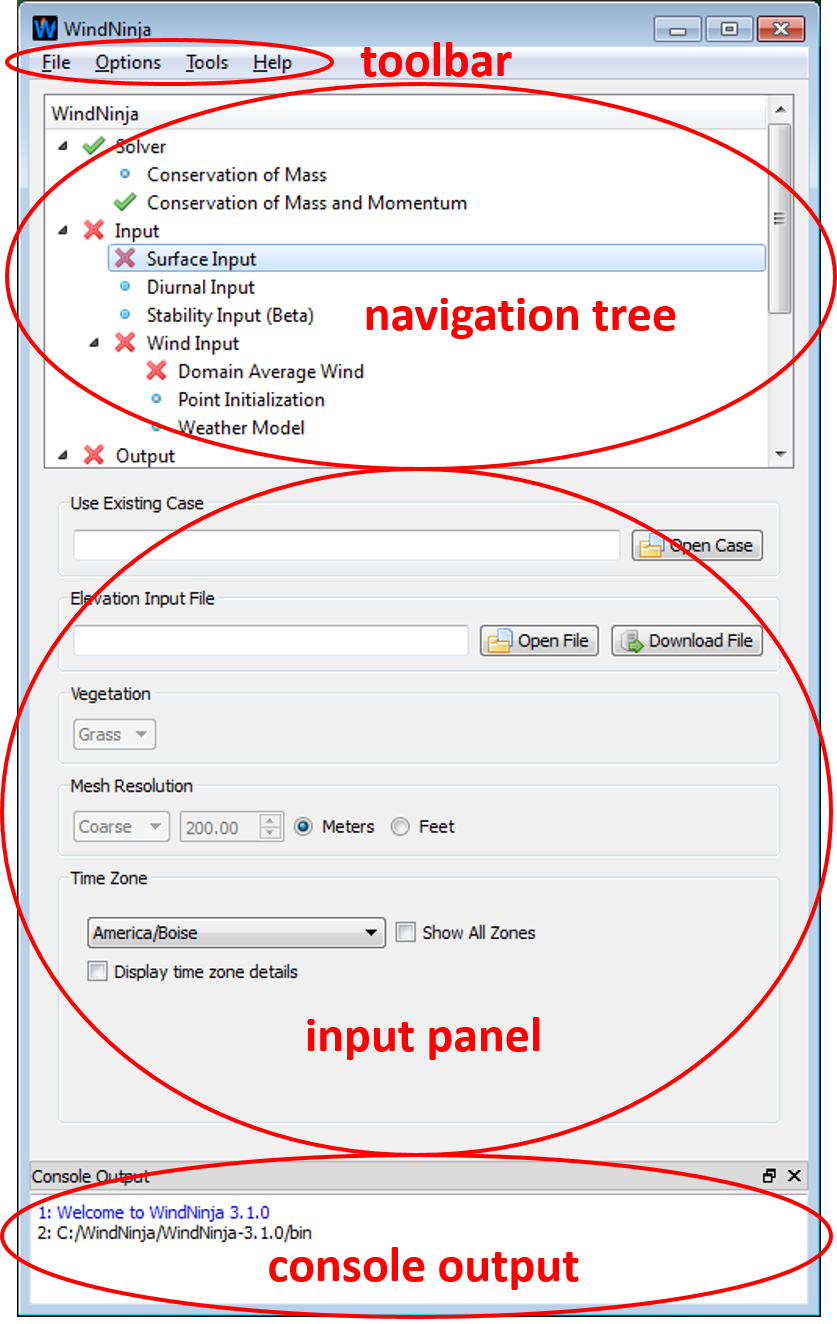
\includegraphics[scale=0.75]{layout_1.png}
\end{figure}

The navigation tree is designed so you can quickly navigate through the process of running a simulation by left-clicking on an element of the tree.  The navigation tree is organized to lead you through the steps of setting up the simulation in logical order, working from top to bottom.  The icons next to each level of the tree indicate the current status of that level.  A 
\includegraphics[scale=0.75]{blue_dot} icon indicates that no selection has been made.  A 
\includegraphics[scale=0.75]{red_cross}  means that either there was a problem with one of your inputs or you have not made a selection at this level yet, but a selection is required.  A 
\includegraphics[scale=0.75]{green_check}  means that your selection for this level in the tree is good.  And a 
\includegraphics[scale=0.5]{ftfo} is a warning that your inputs may not be good but WindNinja cannot determine for sure.  Note that this is just a warning, the simulation may still run fine but you should double check these inputs as WindNinja thinks there may be a problem.  A useful feature of the navigation tree is that you can hover the mouse over anything for additional, specific information about problems, etc.

The input panel is where you actually enter information.  When you select a different part of the navigation tree, the input panel will change allowing you to enter the necessary information.

The console output provides you with feedback from WindNinja.  It’s a good idea to watch this output during your setup and run, especially if there are problems with the run.  Bad problems are usually shown in red text.

\section{Solver}
The solver is the number-crunching part of WindNinja. Starting in WindNinja 3.0 there are two solver options in the navigation tree: 1.) conservation of mass and 2.) conservation of mass and momentum. The conservation of mass option is the native, fast-running solver used in previous versions of WindNinja. The conservation of mass and momentum option is a new solver based on the OpenFOAM toolkit. 


\textbf{\color{red}In the navigation tree, left-click on the solver you want to use under “Solver.” Left-click the box next to the solver name in the input panel to choose the solver.}

\begin{figure}[H]
	\centering
	\label{}
	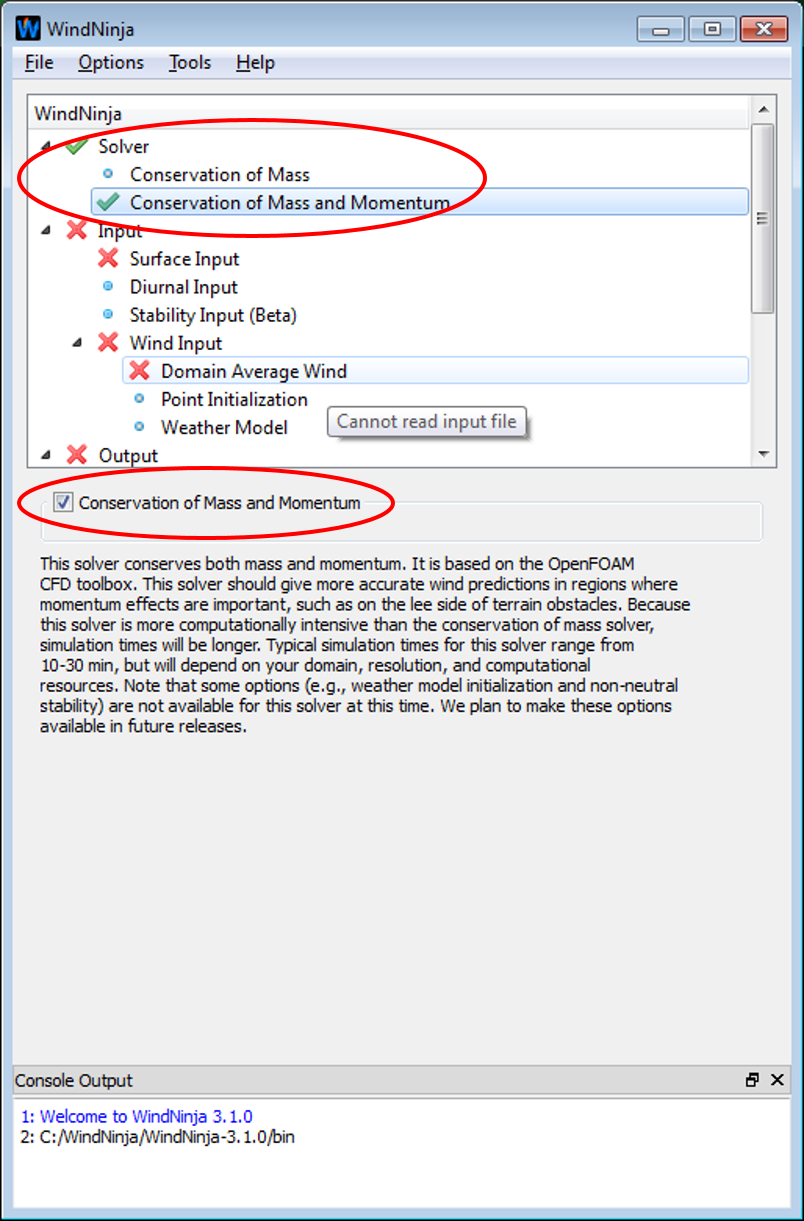
\includegraphics[scale=0.9]{layout_2.png}
\end{figure}

The conservation of mass and momentum solver should give more accurate results than the conservation of mass solver in regions where momentum effects are important, such as on the lee-side of terrain obstacles; however, simulation times will be longer. Typical simulation times for the mass and momentum solver will be on the order of 10-30 min. Note that some options, including weather model initializations and non-neutral stability, are not currently available for the momentum solver. Unavailable options will not be selectable in the navigation tree.

\section{Input}
\subsection{Surface Input}

\textbf{\color{red}In the navigation tree, left-click on “Surface Input”.}

\begin{figure}[H]
	\centering
	\label{}
	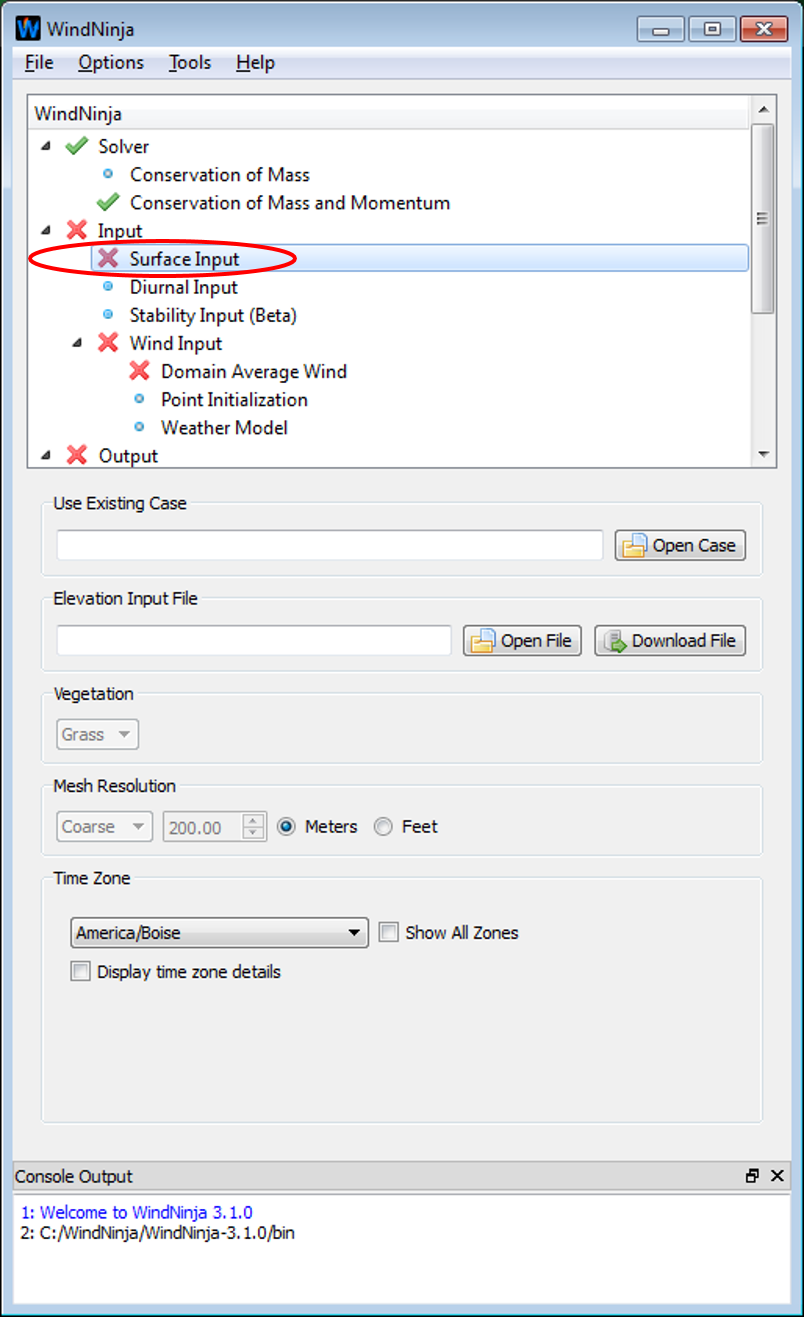
\includegraphics[scale=0.82]{layout_3.png}
\end{figure}

\subsubsection{Obtaining and Specifying the Elevation File}

WindNinja uses an elevation file to obtain the necessary elevation information to simulate wind flow for your specific area.  Several elevation file formats can be read into WindNinja.  They are:

\begin{itemize}
\item[]ASCII Raster (*.asc)
\item[]FARSITE landscape file (*.tif or *.lcp)
\item[]GeoTiff (*.tif)
\item[]ERDAS IMAGINE (*.img)
\end{itemize}

If you already have one of these files for your area, then you can load it, but be sure it meets WindNinja's requirements (described below).  If you don't have an elevation file for your area, you can use the built in file fetching ability of WindNinja to download a file from a USGS or the OpenTopography server.  This feature is very easy to use, and the files conform to WindNinja's requirements.  The document called \href{https://weather.firelab.org/windninja/tutorials/download_elevation_file.pdf}{\texttt{download\_elevation\_file.pdf} } explains this.

If you are just practicing right now, you can also use an elevation file provided by the WindNinja installation.They can be found by going to Start$\Rightarrow$Programs$\Rightarrow$WindNinja-3.0-Example Files.  
In the file browser that opens, you will see the elevation files called \texttt{missoula\_valley.tif}, and \texttt{example\_lcp.lcp} Either of these can be used.

Although all of the elevation file formats mentioned above work in WindNinja, there are some slight differences that deserve explanation.  The ASCII Raster (*.asc) file type is the most common one used in wildland fire, since it is used in the popular fire behavior programs.  So if you will need the elevation file for fire behavior programs in addition to WindNinja, this would probably be the preferred format.  There are two slight disadvantages of this file format: it is a much larger file than the others (ascii and uncompressed), and it's projection/datum information is specified in a separate file (*.prj) that must be in the same folder.  Both the GeoTiff (*.tif) and ERDAS IMAGINE (*.img) file formats are compressed formats that take much less disk space and download time than the ASCII Raster file format.  Also, they contain their projection/datum information in the file rather than a separate file.  If you are only using WindNinja, and not a fire behavior program like FARSITE or FlamMap, either of these would be a good format.  Last, if you already have a FARSITE landscape file (*.tif or *.lcp) because you are doing fire behavior calculations, you should use it because WindNinja will use the canopy and fuels information to infer gridded surface roughness values (surface drag due to vegetation) and heat flux parameters (for a diurnal flow or non-neutral stability simulation).  For the other file formats, you must enter a single, spatially constant vegetation value (described later).

To be able to do a wind simulation, WindNinja has certain requirements that elevation files must meet:
\begin{enumerate}
\item There must be projection/datum information associated with the file and the projection must be defined with that north as ``up.'' This is because we use the standard meteorological convention for wind direction where north is assumed as ``up.''
\item The units of your elevation data must be in meters, that is both the vertical (elevation data) and the horizontal (cell resolution/cell size).
\item Your elevation file should not contain NODATA values (more about this below).
\item It should not be too large in its extent.  A good rule of thumb is to keep your domain less than 30 by 30 miles (50 by 50 km).  Larger sizes are possible, but you may run the risk of your computer running out of memory or you may not be resolving the terrain well enough (if the cell size is large).
\end{enumerate}

Note that files downloaded using the built in WindNinja functionality automatically meet these requirements.

A common problem with user provided elevation files is that they contain NO\_DATA values.  These are locations in the elevation file where elevation data doesn’t exist.  There is now a built-in method in WindNinja to attempt to fill these areas.  When the file is loaded, WindNinja will check for NO\_DATA values.  If detected, it will ask you if you want to try to fill them.  If you say yes, WindNinja will use an interpolation/extrapolation method to try to fill the NO\_DATA values.  This is usually successful if there are not too many cells with NO\_DATA.

One common reason that causes NO\_DATA values is when an elevation file is reprojected in a GIS.  When this is done, NO\_DATA values are sometimes generated around the border because of the warping.  The best way to eliminate these is by first obtaining a larger elevation file than you would normally want, reprojecting it, and then clipping out the NO\_DATA values in a GIS.  See the diagram below describing this process, which must be done by someone with GIS skills.  Note again that elevation files downloaded using the built in WindNinja functionality do not have this problem.

\begin{figure}[H]
	\centering
	\label{}
	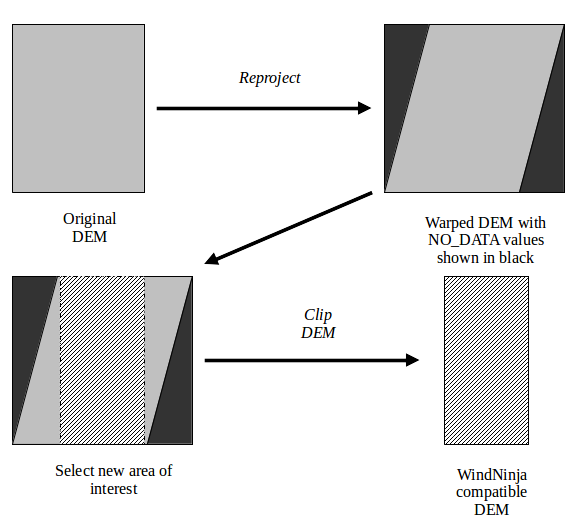
\includegraphics[scale=1.0]{dem_crop.png}
\end{figure}

\textbf{\color{red} With “Surface Input” still selected in the navigation tree, left-click on the “Open Elevation File” button.  In the window that opens, navigate to and select your elevation file.  If you are just practicing, example elevation files are distributed with the WindNinja installation and can be found by going to Start$\Rightarrow$Programs$\Rightarrow$WindNinja-\vn\ $\Rightarrow$Example Files.  You can also download an elevation file by clicking on “Download File.”}


\subsubsection{Using an Existing Case (Conservation of Mass and Momentum Solver)}

Because of the longer simulation times required for the conservation of mass and momentum solver, we provide the option of using an existing case from a previous simulation. This is useful if you do a conservation of mass and momentum simulation and then later want to re-run the same domain at the same resolution, but with a different wind input.

Each time a simulation is run with the conservation of mass and momentum solver, a case directory is left behind in addition to the requested output products.  The name of the case directory will include the word \say{NINJAFOAM}, followed by the name of  your DEM, and a randomly generated number (to prevent overwriting existing case directories). 
For example, a case directory for a simulation using the \say{missoula\_valley.tif}DEM might be named \say{NINJAFOAM\_missoula\_valley\_228391}.

The case directory contains directories and text files which define your case. The case directory can be renamed, but the files within the case directory should not be moved or edited if you plan to reuse the case. The case is linked to the DEM used for the original simulation (usually located in the parent directory of the case directory).

To reuse a case, click \say{Open Case} in the \say{Surface Input} tab. Navigate to the case you would like to use and click “Select Folder.” If WindNinja detects the folder as a valid case, the \say{Use Existing Case} text box will be populated with the case name you selected. WindNinja will look for the corresponding DEM in the parent directory of the specified case and auto-populate the “Elevation Input File” text box if the DEM is found. If the DEM is not found in this parent directory, you will need to select “Open File” and navigate to and select the appropriate DEM.  Note that you cannot change the mesh resolution since the mesh from the existing case is re-used.    

If an existing case is used, the computational domain (the mesh) from the existing case is used for the new simulation. This can reduce the total simulation time by up to 40\%.

\subsubsection{Setting the Dominant Vegetation Type}

WindNinja approximates the drag effect that vegetation has on wind flow in a very simple way.  This requires basic information about the vegetation in the modeling area.  If you used a FARSITE landscape file (*.lcp) for the elevation file, then WindNinja will use the canopy and fuels information in the landscape file to infer the vegetation drag information.  No vegetation input is required by you.  But, if you are using another elevation file type (*.asc, *.tif, or *.img), then you have to choose the dominant vegetation type for your area.  This choice of vegetation type is assumed to prevail over the whole domain.  The choices for vegetation type are:  grass, brush, and trees.  For areas with mixed vegetation types, users should choose the dominant one (meaning the vegetation type that covers most of the domain).

\textbf{\color{red} With “Surface Input” still selected in the navigation tree, select the dominant vegetation type in the input panel using the “Vegetation” drop down list.  If your elevation file was a FARSITE landscape file, this drop-down box will be grayed out, since the vegetation information is obtained from the landscape file.  In this case, you do not need to select a vegetation type.}

\subsubsection{Choosing the Mesh Resolution}

The mesh resolution selection controls the resolution of the wind simulation.  There are four choices for mesh resolution: Coarse, Medium, Fine, and Custom.  The finer the mesh, the longer your simulation will take but smaller undulations in the terrain will be better resolved.  A good default choice for mesh resolution is “Fine”.  The “Custom” selection allows users to enter a specific resolution.  Care should be taken when using “Custom” not to enter too fine of a resolution or your computer could run out of memory.  Typically, mesh resolutions less than around 70-100 meters are too fine and not recommended.  Approximate time estimates for a common sized domain (about 20 miles by 20 miles) using today’s average laptop or desktop computer are shown in the table below. Note that the “Custom” option is not currently available for the conservation of mass and momentum solver. 

\begin{table}[]
\centering
\caption{Simulation times for different mesh resolutions.}
\label{res_table}
\begin{tabular}{lll}
\toprule
\multirow{2}{*}{Resolution} & \multicolumn{2}{l}{Approximate Time} \\ \cmidrule(l){2-3} 
 & Conservation of Mass & Conservation of Mass and Momentum \\ \cmidrule(r){1-1}
Coarse & 10 s & 1 hr \\
Medium & 25 s & 2 hr \\
Fine & 35 s & 3 hr \\ \bottomrule
\end{tabular}
\end{table}

\textbf{\color{red}Select your desired mesh resolution using the \say{Mesh Resolution} drop-down list.}

Notice that if you choose Coarse, Medium, or Fine, the actual resolution of the simulation in meters or feet is displayed in the grayed-out box to the right of the “Mesh Resolution” drop-down list.

\subsubsection{Time Zone}

Time zone information is not required for this tutorial, so you do not need to make a choice here.  Other tutorials that need information about sun angles (diurnal winds and stability calculations) require that a valid time zone be specified.

\subsection{Diurnal Input and Stability Input}
Since no diurnal wind or non-neutral stability will be simulated in this tutorial, no selections need to be made under the “Diurnal Input” or “Stability Input” headings in the navigation tree.  An explanation of these types of simulations is given in WindNinja Tutorial 2: Diurnal Wind and Non-neutral Stability.  For this simulation, a   symbol should be next to “Diurnal Input” and “Stability Input” in the navigation tree indicating no selection has been made.

\subsection{Wind Input}

A basic WindNinja simulation will be done, which means that we will initialize the simulation using a domain averaged wind speed and direction.  Other initialization methods are discussed in later tutorials.

\textbf{\color{red} Under \say{Wind Input} in the navigation tree, left-click on \say{Domain Average Wind}.}

\subsubsection{Input Wind Height}

In WindNinja, users must specify the height of the input domain averaged wind speed and direction (domain averaged wind speed and direction are discussed below in section 3.3.2).  For this height, the meteorological standard is used \textit{where the wind height specified is the height above the top of the vegetation.}  So if the area has 100 foot tall trees, the \say{20-foot wind} is actually 120 feet above the ground surface (20 feet above the tops of the trees).  In this example, the user would choose \say{20 ft} for the WindNinja input wind height.  In the US, the standard height for meteorological measurements in the context of wildland fires is usually 20 feet above the vegetation.  Most RAWS stations measure this 20 foot wind and fire weather forecasts generally specify the 20 foot wind.  FARSITE and FlamMap also use the 20 foot wind.  One exception in the US to this is METAR weather stations which measure the wind at 10 meters.  Most other countries such as Canada, Australia, etc. use 10 meters as the standard wind measurement height.

\textbf{\color{red} Select your input wind height using the “Input Wind Height” drop down list.}

Note that a “custom” height can also be entered manually.

\subsubsection{Entering the Input Wind Speed and Direction}

Terrain causes changes in wind speed as air flows over it.  Directional changes also occur due to channeling of the flow.  For a  domain average initialized run, WindNinja requires you to enter a single wind speed and direction to characterize the wind field for the particular wind scenario you are trying to simulate.  This input wind speed and direction can be thought of as roughly an average surface wind over the simulation domain at the input height.  So if you want a particular wind speed at, say, a certain ridge top, you will have to adjust your input wind speed and direction accordingly.  This means that you may have to run multiple simulations varying the input speed and direction to get the resulting wind that you want at that particular ridge top.

There are many resources that you can use to help determine good wind speeds and directions to enter, depending on your specific circumstances.  For example, if you are on a fire and want to predict winds for tomorrow, you could look at the general weather forecast or a spot weather forecast and use the \say{Lower Elevation} or \say{Ridgetop Wind} predictions to guide your WindNinja inputs.  Or if you are on a fire with homes or other valuable resources on one side of the fire, you could do \say{what-if} types of wind runs to help determine what would happen if the wind pushed the fire in that direction.  Similar \say{what-if} wind runs could be done for planning of prescribed fires.  Also, measured winds from RAWS stations or observers could be used to reconstruct a past fire.  Several other scenarios are possible…

WindNinja follows the meteorological convention that the wind direction is the direction that the wind is coming from (so a $270^{\circ}$  wind blows from west to east).  WindNinja also lets you choose the units of your input and output wind speed.

As a convenience, you can enter many different input wind speed and direction combinations at the same time and then run all of these simulations at once.  Output files will be written for each speed and direction combination.

\textbf{\color{red} With \say{Domain Average Wind} still selected in the navigation tree, enter your desired wind speed and direction in the \say{Speed} and \say{Direction} text boxes.  You may enter multiple combinations, row by row.  Also select your preferred wind speed units at the top of the speed list.}

In this panel, you have probably noticed that there are also columns to the right, such as \say{Time}, \say{Date}, etc. that are grayed out.  These are all related to diurnal and non-neutral stability wind simulations, which are explained in WindNinja Tutorial 2: Diurnal Wind and Non-neutral Stability.  They can be ignored for now.

\section{Output}

WindNinja writes many different kinds of output files for use in a GIS, Google Earth, fire modeling programs, and engineering programs.  The following sections describe how to identify and work with these output files.  \textit{Note that output files are written to the folder where your elevation file is located.} The files are automatically named based on your input parameters.  Here we will describe the file naming convention used by WindNinja for a domain average initialized run.  Other types of runs will have slightly different naming conventions and are discussed in other tutorials.

The naming convention includes a combination of the elevation file name, input wind direction, input wind speed and output file resolution.  Below is an example of the output files from a WindNinja run using an ASCII Raster elevation file called \say{south\_canyon.asc} and an input direction of 270 degrees and speed of 35 mph with an output file resolution of 200 meters.

\begin{figure}[H]
	\label{}
	\centering
	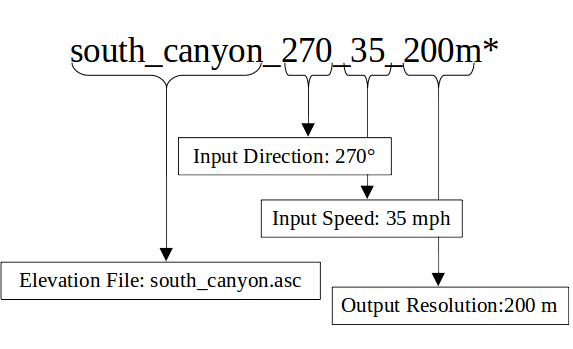
\includegraphics[scale=1.0]{file_desc}
\end{figure}

A total of 14 files may share this base name with different appendages and file extensions (indicated above by the (*) asterisk).  The table below describes each file.
\newline

\begin{center}
% \usepackage{multirow}


\begin{tabular}{|l|l|} 
\hline
\textbf{File}                          & \textbf{Description}                                     \\ 
\hline
south\_canyon.asc                      & Input elevation file                                     \\ 
\hline
south\_canyon.prj                      & Projection file associated with the elevation file       \\ 
\hline
south\_canyon\_270\_35\_200m.shp       & \multirow{3}{*}{Shape files created for ArcView/ArcMap}  \\ 
\cline{1-1}
south\_canyon\_270\_35\_200m.shx       &                                                          \\ 
\cline{1-1}
south\_canyon\_270\_35\_200m.dbf       &                                                          \\ 
\hline
south\_canyon\_270\_35\_200m.prj       & Shape files projection file                            \\ 
\hline
south\_canyon\_270\_35\_200m.kmz       & Google Earth File                                        \\ 
\hline
south\_canyon\_270\_35\_200m\_vel.asc  & FARSITE/FlamMap grid for wind speed                      \\ 
\hline
south\_canyon\_270\_35\_200m\_vel.prj  & FARSITE/FlamMap wind speed projection file               \\ 
\hline
south\_canyon\_270\_35\_200m\_ang.asc  & FARSITE/ FlamMap grid for wind direction                 \\ 
\hline
south\_canyon\_270\_35\_200m\_ang.prj  & FARSITE/FlamMap wind direction projection file           \\ 
\hline
south\_canyon\_270\_35\_200m\_cld.asc  & FARSITE/ FlamMap grid for cloud cover                    \\ 
\hline
south\_canyon\_270\_35\_200m\_cld.prj  & FARSITE/FlamMap cloud cover projection file              \\ 
\hline
south\_canyon\_270\_35\_200m.atm       & FARSITE atmosphere file                                  \\ 
\hline
south\_canyon\_270\_35\_200m\_surf.vtk & Paraview/VTK surface file                                \\ 
\hline
south\_canyon\_270\_35\_200m.vtk       & Paraview/ VTK volume data file                           \\
\hline
\end{tabular}
\end{center}

Just like the input wind height in Section 3.3.1, you must choose the output wind height and speed units that you would like.  This is the height and speed units that winds in the output files are reported at.

\textbf{\color{red} In the navigation tree, left-click on “Output”.  Then in the inputs panel, select the “Output Height” and “Output Speed Units” you desire using the drop down list.}

There is a feature in WindNinja that allows users to “clip” off a border area around your output files.  The intent of this feature is to let you automatically clip off border areas that might be less accurate because of their close proximity to the boundary of the domain.  Typically this boundary influence might extend 5-10\% in from the border of the domain, although users normally don't use this feature and commonly just leave the default value of 0\%.

\subsection{Google Earth}

Probably the most convenient way to view winds from WindNinja is to use Google Earth.

\textbf{\color{red} To write Google Earth files using WindNinja, select \say{Google Earth} in the navigation tree.  Then check the \say{Create Google Earth Files} check box in the input panel.}

Notice that there are several options to control how the wind vectors will look in Google Earth.  The default values work well, and don't normally need to be changed.  If you want to, you can change the line width of the plotted wind vectors using the \say{Line Width} text box.  You can also adjust the wind speed legend by choosing either \say{Uniform Range} or “Equal Count”.  This affects where the speed \say{breaks} are in the legend between different colors.  \say{Uniform Range} sets the speed \say{breaks} in the legend uniformly in speed among the entire range of speeds.  \say{Equal Count} means that the speed \say{break} for each wind vector color will be set so that there are equal numbers of red, orange, yellow, etc. vectors displayed.  The resolution of the Google Earth output file can be set in the \say{Resolution} area.  By default, the WindNinja mesh resolution is used, which is displayed in the grayed out text box.  You can uncheck the \say{Use Mesh Resolution} check box to specify your own resolution.  Be careful to not specify too fine of a resolution, since the graphics in Google Earth may be very slow or Google Earth could crash.  A good rule of thumb is to keep the resolution greater than about 100 meters.

Once WindNinja has computed the wind output files (after the solve step explained below in Section 5), you can view the Google Earth output file (*.kmz) in Google Earth.  To do this, you must first have Google Earth installed on your computer (it’s a free download from \url{http://earth.google.com/}).  Then just double-click on the *.kmz file (located in the same folder as your elevation file) that was created by WindNinja and Google Earth will automatically start up, load the wind file, and zoom into the area you simulated. An example screen capture of winds viewed in Google Earth is shown below.  The wind layer can be turned on and off using the check box in the “Places” panel on the left of the Google Earth window.

\begin{figure}[H]
	\label{}
	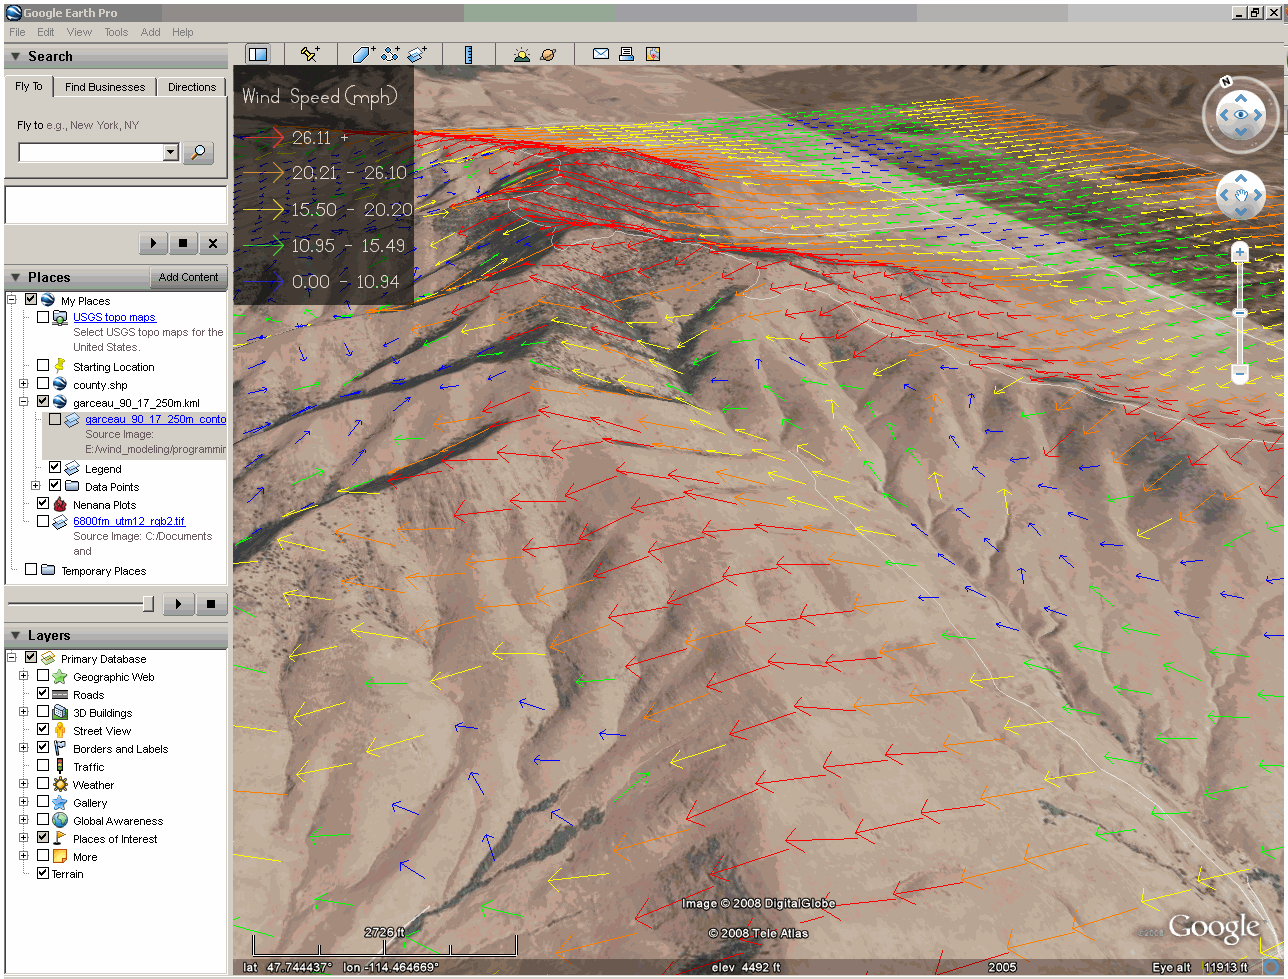
\includegraphics[scale=0.35]{earth_1}
\end{figure}

\subsection{Fire Behavior}
WindNinja writes wind files that can be used in FARSITE and FlamMap for fire behavior simulations.  Spatially varying winds like those produced by WindNinja are often termed gridded winds in these programs.

The WindNinja files for use in FARSITE and FlamMap are ASCII Raster format, the same format as the other files used for elevation, fuels, etc. in these programs.  There are three gridded files created by WindNinja:  a wind speed file (*\_vel.asc), a wind direction file (*\_ang.asc), and a cloud cover file (*\_cld.asc).  Each file also has a corresponding projection file (*.prj).  Cloud cover is not simulated in WindNinja, but is a required file for running FARSITE using gridded winds.  As a convenience, WindNinja provides a cloud cover file with 0\% cloud cover to facilitate gridded wind simulations in FARSITE if cloud cover information is not available.  You could change this for your FARSITE simulation by opening the cloud cover file in a text editor and changing the zero to another value.

It is simple to run FlamMap using gridded winds.  Just select the \say{Wind Vectors} radio button where you normally enter wind information in FlamMap.  Then choose the \say{Direction} file and the \say{Speed} file.  These correspond to the WindNinja \say{*\_ang.asc} and \say{*\_vel.asc} files, respectively.

To use gridded winds in FARSITE, you must use an \say{atmosphere file} (*.atm).  WindNinja can make this file for you.  The atmosphere file specifies wind file names to be used over time in the FARSITE simulation, since a FARSITE simulation steps through time.  In this way, different wind files can be used at different times during the fire simulation.  The atmosphere file—a text file specifying month, day, hour, wind speed filename, wind direction filename, and cloud cover filename—must be precisely formatted to function in FARSITE and in the same folder as the wind speed, wind direction, and cloud cover files.  You can find more information about using gridded wind in the FARSITE Help by searching for “Gridded Weather File”.

\textbf{\color{red} To make fire behavior output files, left-click on “Fire Behavior” in the navigation tree.  Then check the “Create Fire Behavior Files” check box.}

The resolution of the fire behavior files can be set here.  By default, the WindNinja mesh resolution is used, with the actual value displayed in the grayed out text box.  You can uncheck the \say{Use Mesh Resolution} check box to specify your own resolution.  Be careful to not specify too fine of a resolution.  A good rule of thumb is to keep the resolution greater than about 100 meters.

You can also select if you want to create a FARSITE atmosphere file (*.atm) here.

\subsection{Shape Files}
Shapefiles for viewing simulated wind in a GIS are created by WindNinja.  Four files (*.shp, *.shx, *.dbf, *.prj) are made for viewing in ArcMap, ArcView, or Quantum GIS.  These files are always in the same projection as the elevation file and created in the same directory.  To view wind vectors in ArcMap or ArcView, you can follow the instructions for \href{https://weather.firelab.org/windninja/tutorials/ArcGIS.pdf}{ArcMap} or \href{http://firelab.github.io/windninja/pdf/displaying_wind_vectors_in_ArcView.pdf}{ArcView}.

\textbf{\color{red} To make shape files, left-click on \say{Shape Files} in the navigation tree.  Then check the \say{Create Shape Files} check box.}

The resolution of the shape files can be set here.  By default, the WindNinja mesh resolution is used, with the actual value displayed in the grayed out text box.  You can uncheck the \say{Use Mesh Resolution} check box to specify your own resolution.  Be careful to not specify too fine of a resolution.  A good rule of thumb is to keep the resolution greater than about 100 meters.

\textbf{\color{red} Select the desired output resolution.}

\subsection{Geospatial PDF Files}

Geospatial PDF files are geospatially referenced PDF files. They can be viewed in regular PDF viewers as well as in GIS programs and the Avenza PDF Maps mobile application. 

\textbf{\color{red} To make Geospatial PDF output files, left-click on \say{Geospatial PDF Files} in the navigation tree.  Then check the \say{Create Geospatial PDF Files} check box.}

There are two options for the basemap, a simple hillshade and a TopoFire topographical map that includes roads, boundaries, etc. The PDF can be printed in either portrait or landscape layout.

\textbf{\color{red} Select the desired basemap and layout.}

The resolution of the Geospatial PDF files can be set here.  By default, the WindNinja mesh resolution is used, with the actual value displayed in the grayed out text box.  You can uncheck the \say{Use Mesh Resolution} check box to specify your own resolution.  Be careful to not specify too fine of a resolution.  A good rule of thumb is to keep the resolution greater than about 100 meters.

\textbf{\color{red} Select the desired output resolution.}

\subsection{VTK Files}

VTK output files can be used in scientific and engineering programs to view the full 3-d output wind fields.  These programs are fairly complex, and will likely not be used very often by fire analysts and managers.  One program to view these files is the free, open-source program \href{http://www.paraview.org/}{ParaView} by \href{http://www.kitware.com/}{Kitware, Inc.}  This program allows users to view the full 3-d wind fields simulated by WindNinja, as opposed to all the other types of output files and viewers discussed earlier where only 2-d surface winds can be viewed.  In ParaView, you have the ability to use several advanced viewing capabilities such as user defined 2-d slices, raster and vector plotting, contour plotting, and plotting of the computational grid.

The two VTK files produced by WindNinja are the full 3-d volume data and a ground surface file.  We will not produce these files for this tutorial.

Note that VTK files are not available for the momentum solver.

\section{Solve}

Now you've entered all the required inputs and are ready to run the simulation(s).  WindNinja has the ability to use multiple processors/cores if your machine has them.  This can dramatically reduce the simulation time.

\textbf{\color{red} Left-click on \say{Solve} in the navigation tree.  Set the number of processors you would like using the \say{Number of Processors} text box.  Notice that the number of available processors on your computer is detected and displayed.  Finally, left-click the \say{Solve} button to start the simulation(s).}

\begin{figure}[H]
	\label{}
	\centering
	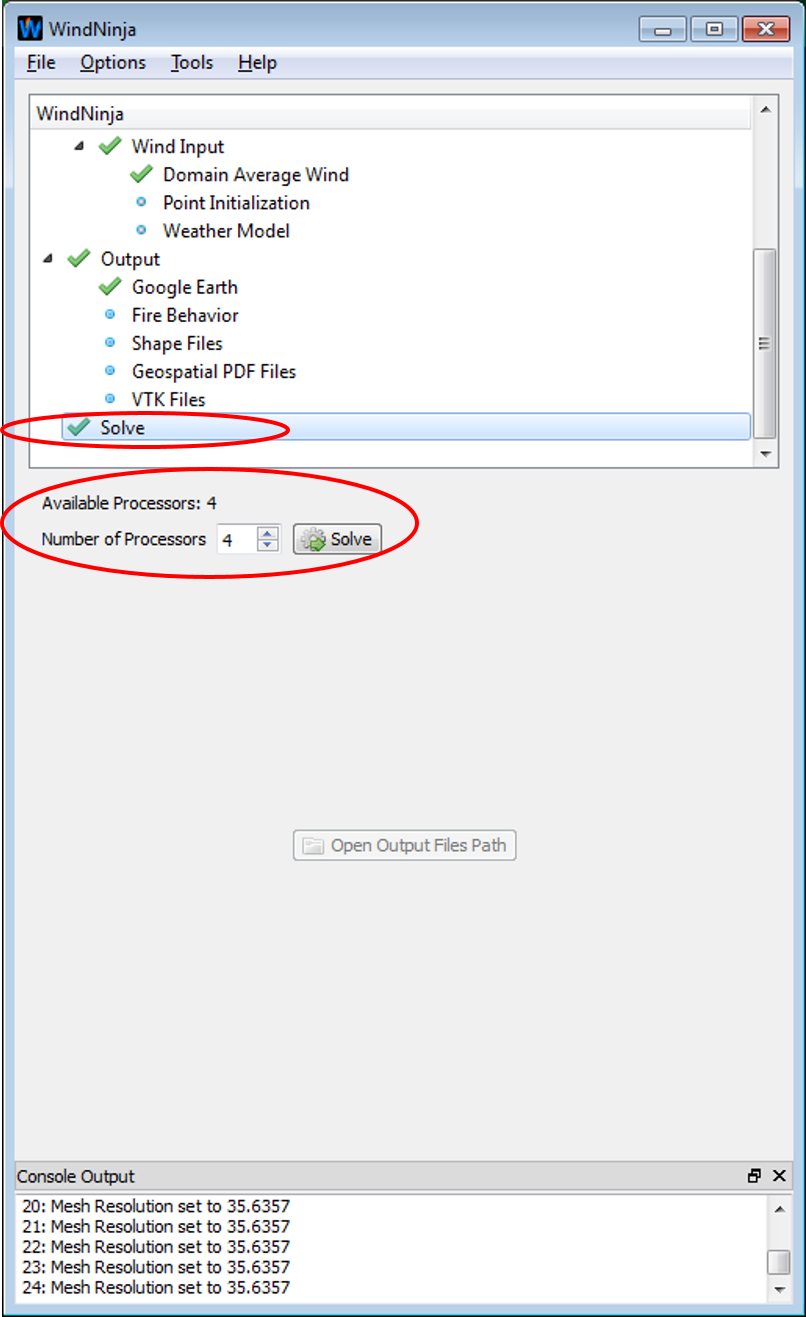
\includegraphics[scale=1.0]{solve_1}
\end{figure}

A progress window will open (this may take a few seconds) that displays how far along the simulation is.  When the simulation is done, the progress bar will notify you.

\textbf{\color{red} Click \say{Close} in the progress window.}

\begin{figure}[H]
	\label{}
	\centering
	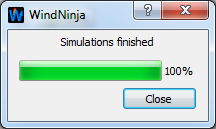
\includegraphics[scale=1.0]{sim_finished_1}
\end{figure}

The simulations are complete!  The output files can be found in the folder where your elevation file is.  For your convenience, a button on the solve input panel called \say{Open Output Files Path} can be clicked to open your file browser in the folder where the output files were written.

\textbf{\color{red} Left-click the \say{Open Output Files Path} button to see the output files that were written.}

\begin{figure}[H]
	\label{}
	\centering
	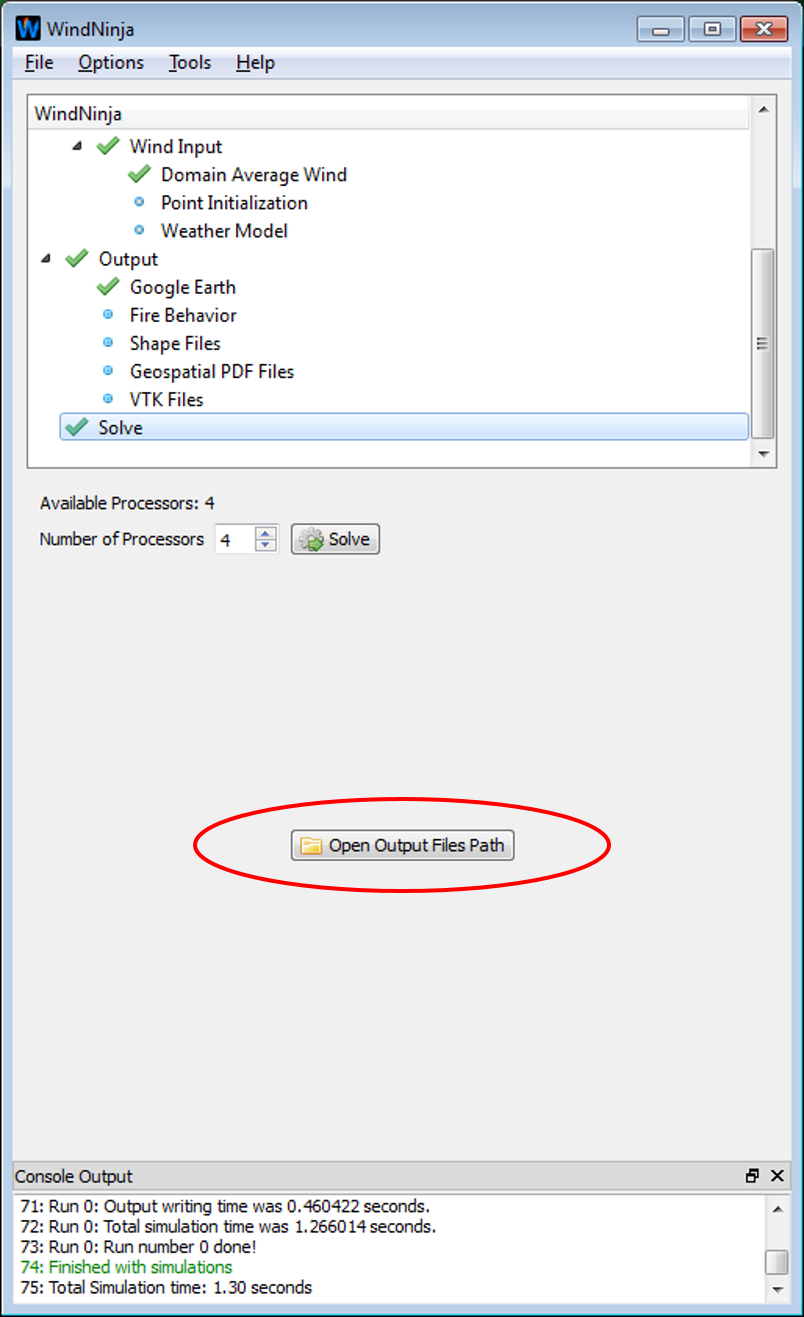
\includegraphics[scale=1.0]{output_path_1}
\end{figure}

This concludes \textbf{WindNinja Tutorial 1: The Basics}.  You are encouraged to do the other tutorials that are available.

\section{Advanced Users}

Advanced users should note that the default settings in WindNinja have been selected to ensure fast run times for operational wildland fire applications. In some cases this may mean trading slightly higher accuracy for computational efficiency.  Advanced users can modify many of these options via the WindNinja command line interface (CLI). The CLI is described in \href{https://weather.firelab.org/windninja/tutorials/CLI_instructions.pdf}{CLI\_instructions.pdf}. The CLI allows for far more customizable WindNinja runs and access to features that are not available in the GUI. Researchers, programmers, and other advanced users are strongly encouraged to explore the capabilities offered in the CLI. The WindNinja source code and additional information can be found at: \url{https://github.com/firelab/windninja}.

\end{document}
